\chapter{Modelling a Memory Box}
\label{chap:membox}

 The toughest part of learning a new language  is often building up a sufficient
vocabulary.  This is usually accomplished by repeating a long list of words
again and again till they stick.  A memory box is a simple but ingenious little
contraption to support this tedious process of memorisation.  As depicted in
Fig.~\ref{fig:membox_illustration}, it consists of a series of compartments or
partitions usually of increasing size.  The content to be memorised is written
on a series of cards  which are initially placed in the first partition.  All
cards in the first  partition should be repeated everyday and cards that have
been successfully  memorised are placed in the next partition.  Cards in all
other partitions are  only repeated when the corresponding partition is full and
cards that are  answered correctly are moved one partition forward in the box. 
Challenging  cards that have been forgotten are treated as brand new cards and
are always  placed right back into the first partition regardless of how far in
the box they  had progressed.  These ``rules'' are depicted by the green and red
arrows in  Fig.~\ref{fig:membox_illustration}. The basic idea is to repeat
difficult cards as often as necessary  and not to waste time on easy cards which
are only repeated now and then to keep them in memory.  The  increasing size of
the partitions represents how words are easily placed in our limited short term
memory and slowly move in our theoretically unlimited long term memory if
practised often enough.
 
%\usepackage{graphics} is needed for \includegraphics
\begin{figure}[htp]
\begin{center}
  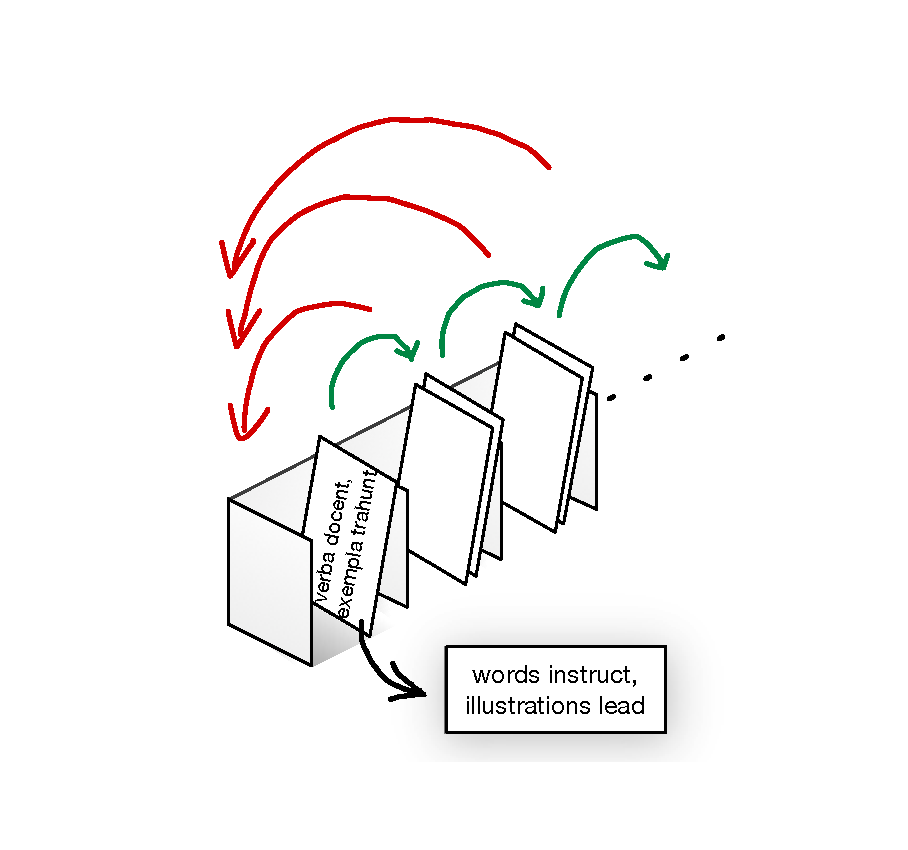
\includegraphics[width=0.4\textwidth]{pics/membox_illustration}
  \caption[]{Possible \emph{Concrete Syntax} of our Memory Box.}
  \label{fig:membox_illustration}
\end{center}
\end{figure}

A memory box is an interesting system, because it consists clearly of a static
structure (the box, partitions and their sizes, cards with their sides and
corresponding content) and a set of rules that describe the dynamic aspects 
(behaviour) of the system.  In the rest of the tutorial we shall build a
complete memory box from scratch in a model-driven fashion and use it to
introduce fundamental concepts in metamodelling and MDSD in general.  

\section{A Language Definition Problem?}

Like in any area of study, metamodelling has its fair share of buzz words used
by experts to communicate concisely.  Although some concepts might seem quite
abstract for a beginner, a well defined vocabulary is important so we know
exactly what we are talking about.   

The first step is understanding that metamodelling equates to language
definition.  This means that the task of building a system like our memory box
can be viewed as defining a suitable language that can be used to describe the
system.  This language oriented approach has a lot of advantages including a
natural support for product lines (individual products are valid members of the
language) and a clear separation between platform independent and platform
specific details.      

So what constitutes a language?  The first question is obviously  how the
building blocks of your language actually ``look'' like.  Is your language to be
textual?  Visual?  This is referred to as the \emph{Concrete Syntax} of a
language and is basically an interface to end users who use the language.  
\marginpar{\emph{Concrete Syntax}}
In the case of our memory box, Fig.~\ref{fig:membox_illustration} can be viewed
as a possible concrete syntax.  As we are however building a memory box as a
software system, our actual concrete syntax  will probably be composed of GUI
elements like buttons, drop-down menus and text fields.   

Irrespective of how a language looks like, members of the language must adhere
to the same set of ``rules''.  
\marginpar{\emph{Grammar}}
For a natural language like English, this set of rules is usually called a
\emph{grammar}.  
In metamodelling, however, everything is represented as a graph of some kind
and, although the concept of a  \emph{graph grammar} is also quite well-spread
and understood, metamodellers  more often use a \emph{type graph} that defines
what types and relations  constitute a language. 
\marginpar{\emph{Graph Grammar}}
\marginpar{\emph{Type Graph}}
A graph that is a member of your language must \emph{conform to} the
corresponding type graph for the language.  To be more precise, it must be
possible to type the graph according to the type graph, i.e., the types and
relations used in the graph must exist in the type graph and not contradict the
structure defined there.  
\marginpar{\emph{Abstract Syntax}}
This way of defining membership to a language has many parallels to the
class-object relationship in the Object Oriented paradigm and should seem very
familiar for any programmer used to OO.  This type graph is referred to as the
\emph{Abstract Syntax} of a language. 

Very often, one might want to further constrain a language, beyond simple typing
rules.  
\marginpar{\emph{Static Semantics}}  
This can be accomplished with a further set of rules or constraints that
members of the language must fulfil in addition to being conform to the type
graph.
These further constraints are referred to as the \emph{Static Semantics}
of a language.    

With these few basic concepts, we can now introduce a further and central
concept in metamodelling, the \emph{metamodel} (basically a simple class
diagram). 
\marginpar{\emph{Metamodel}}
A metamodel defines not only the abstract syntax of a language but also some
basic constraints (a part of the static semantics).  
Thinking back to our memory box, we could define the types and relations we want
to allow, e.g.,  a box with partitions, cards, the box contains partitions that
contain cards. 
Multiplicities are an example for constraints that are no longer part of the
abstract syntax and belong to static semantics, but can nonetheless be expressed
in a metamodel.
For example, that a card can only be in one partition, or that a partition has
only one next partition or none.
\marginpar{\emph{Constraint Language}}  
More complex constraints that cannot be expressed in a metamodel are usually
specified using an extra \emph{constraint language} such as OCL (the Object
Constraint Language).
This goes beyond this tutorial however and we'll stick to metamodels without
using an extra constraint language.              

$\textbf{A short recap:}$  we have learnt that metamodelling starts with
defining a suitable language.  
For the moment, we know that a language comprises a concrete
syntax (how does the language look like),  an abstract syntax (types and
relations of the underlying graph structure), and static semantics (further
constraints that members of the language must fulfil).
Metamodels are used to define the abstract syntax and a part of the static
semantics of a language, while \emph{models} are graphs that conform to some
\marginpar{\emph{Model}}
metamodel (can be typed  according to the abstract syntax and adhere to the
static semantics). 

This tutorial is meant to be be hands-on so enough theory!  Lets
define, step-by-step, a metamodel for our memory box using our tool eMoflon.  
  
\section{Abstract Syntax and Static Semantics}

Switch to EA, choose \texttt{Demo} and click on the button \texttt{Add a
Package} as depicted in Fig.~\ref{fig:new_package}.   

\begin{figure}[htbp]
	\centering
  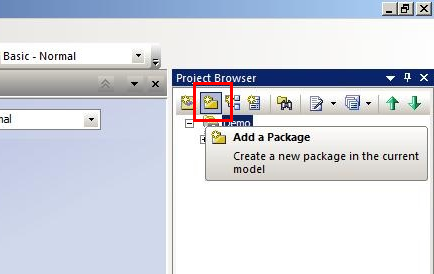
\includegraphics[width=0.5\textwidth]{pics/memBoxBilder/memBox01.png}
	\caption{Add a new package to \texttt{Demo}.}
	\label{fig:new_package}
\end{figure} 

In the dialogue that pops up (Fig.~\ref{fig:new_package_name}), choose
\texttt{Class View}, enter \texttt{Memory\-Box\-Language} as the name of the new
package and click \texttt{OK}. 

\begin{figure}[htbp]
	\centering
    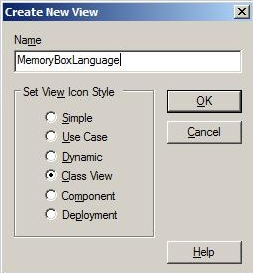
\includegraphics[width=0.3\textwidth]{pics/memBoxBilder/memBox02.png}
	\caption{Enter the name of the new package.}
	\label{fig:new_package_name}
\end{figure}

In your EA workspace the \texttt{Project Browser} should now look like
Fig.~\ref{fig:new_package_completed}.

\begin{figure}[htbp]
	\centering
  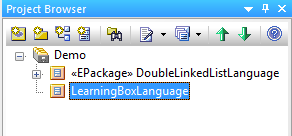
\includegraphics[width=0.5\textwidth]{pics/memBoxBilder/memBox03.png}
	\caption{State after creating the new package.}
	\label{fig:new_package_completed}
\end{figure}

\clearpage 

Now click the button \texttt{New Diagram} (Fig.~\ref{fig:diagram}).

\begin{figure}[htbp]
	\centering
  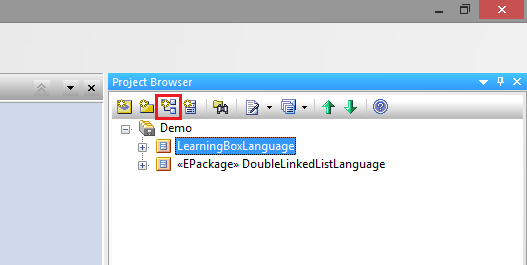
\includegraphics[width=0.7\textwidth]{pics/memBoxBilder/memBox04.png}
	\caption{Add a diagram.}
	\label{fig:diagram}
\end{figure}

In the dialog that pops up (Fig.~\ref{fig:diagram_type}), choose \texttt{Ecore
Diagram} and  \texttt{OK}. 


\begin{figure}[htbp]
	\centering
  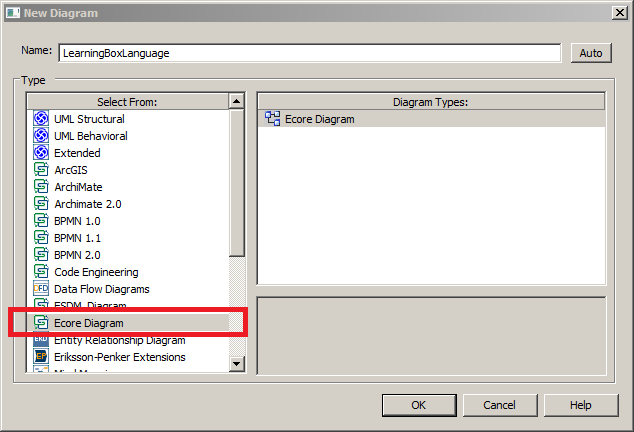
\includegraphics[width=0.8\textwidth]{pics/memBoxBilder/memBox05.png}
	\caption{Choose type of diagram.}
	\label{fig:diagram_type}
\end{figure}

In analogy to the ``everything is an object''
principle in the OO paradigm, in metamodelling, everything is a model.
\marginpar{\emph{Unification}}
This principle is called \emph{Unification} and has a lot of advantages.
If everything is a model, a metamodel that defines (at least a part of) a
language must be a model itself.
\marginpar{\emph{Meta-metamodel}}
\marginpar{\emph{Meta-Language}}
\marginpar{\emph{Modelling Language}}
This means that it conforms to some \emph{meta-metamodel} which defines a
\emph{(meta)modelling language} or \emph{meta-language}.
For metamodelling with eMoflon, we support \emph{Ecore} as a modelling language
and it defines types like \texttt{EClass} and \texttt{EReference}, which we will
be using to specify  our metamodels.
Other modelling languages include MOF, UML and Kermeta. 

\clearpage

After creating the new diagram, your  \texttt{Project Browser} should now
resemble Fig.~\ref{fig:diagram_completed}.  Double-click the newly
created diagram to ensure that it is open.

\begin{figure}[htbp]
	\centering
  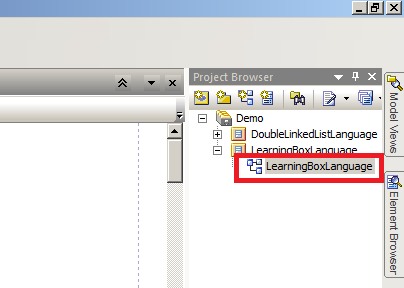
\includegraphics[width=0.7\textwidth]{pics/memBoxBilder/memBox06.png}
	\caption{State after creating diagram.}
	\label{fig:diagram_completed}
\end{figure}

To the left of the workbench in EA, a \emph{Toolbox} should have appeared
containing the types available in Ecore for metamodelling
(Fig.~\ref{fig:eclass}).  Click on \texttt{EClass} and click in the open
diagram (the main window in EA).

\begin{figure}[htbp]
	\centering
  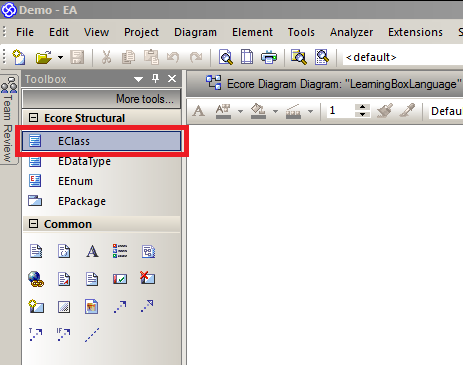
\includegraphics[width=0.7\textwidth]{pics/memBoxBilder/memBox07.png}
	\caption{Create an EClass.}
	\label{fig:eclass}
\end{figure}

\clearpage

In the dialogue that pops-up, enter \texttt{Box} as the name of the class and
click \texttt{OK} (Fig.~\ref{fig:eclass_properties}).  This dialogue can
always be invoked by double-clicking the class and contains many other
properties we'll be looking into later in the tutorial.  In general, a similar
``properties'' dialogue can be opened in the same fashion for almost every
element in EA.

\begin{figure}[htbp]
	\centering
  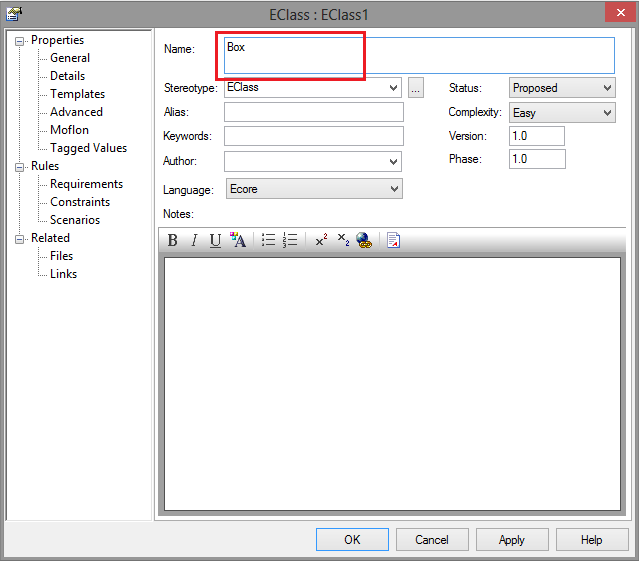
\includegraphics[width=0.6\textwidth]{pics/memBoxBilder/memBox08.png}
	\caption{Enter properties of EClass.}
	\label{fig:eclass_properties}
\end{figure}

After creating \texttt{Box}, your EA workspace should resemble
Fig.~\ref{fig:eclass_completed}. 

\begin{figure}[htbp]
	\centering
  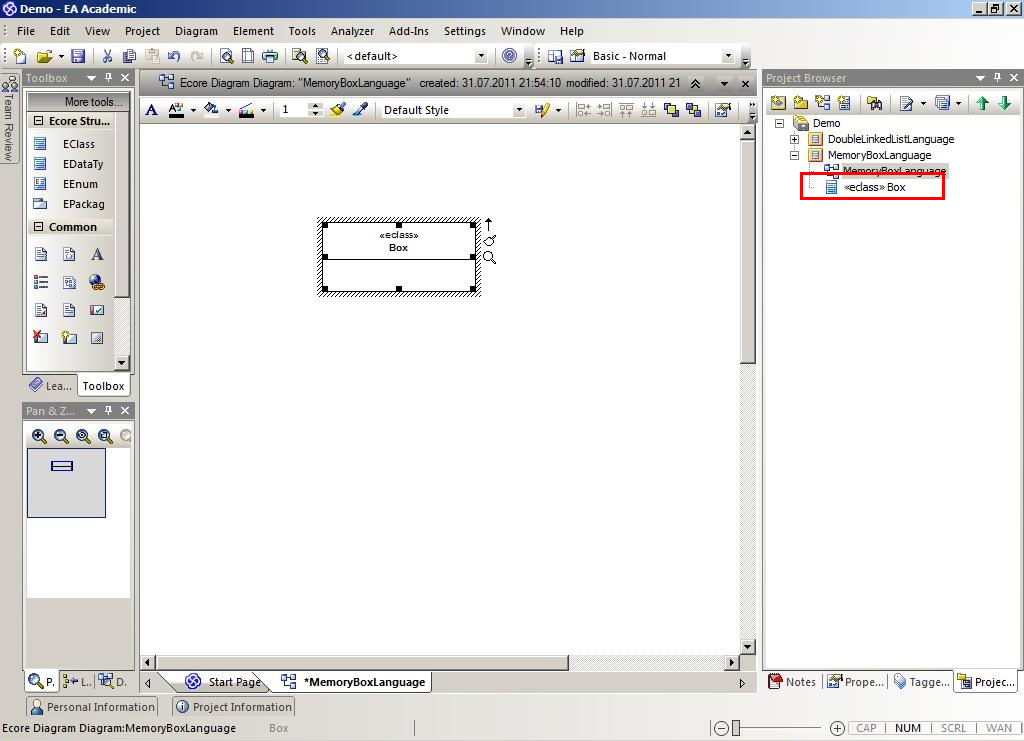
\includegraphics[width=0.7\textwidth]{pics/memBoxBilder/memBox09.png}
	\caption{State after creating \texttt{Box}.}
	\label{fig:eclass_completed}
\end{figure}

\clearpage

Now create \texttt{Partition} and \texttt{Card} in the same way, till your
workspace resembles Fig.~\ref{fig:all_eclasses}.  These are the main classes for
our memory box.

\begin{figure}[htbp]
	\centering
  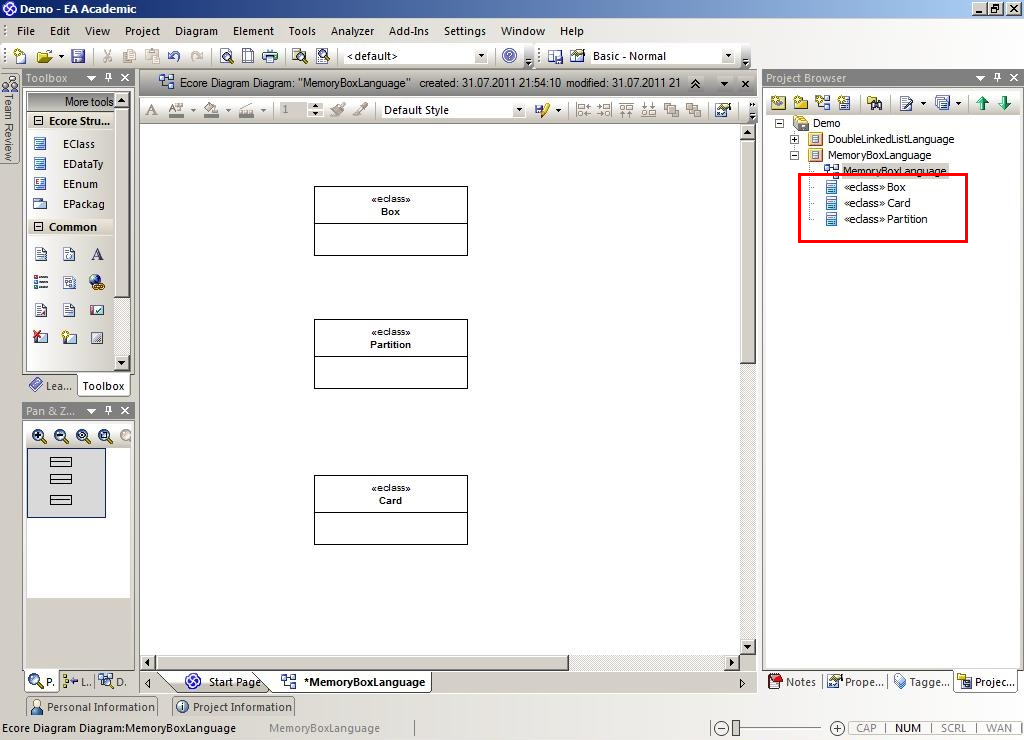
\includegraphics[width=0.7\textwidth]{pics/memBoxBilder/memBox10.png}
	\caption{Main classes in our metamodel.}
	\label{fig:all_eclasses}
\end{figure}

Now choose \texttt{Box}, right-click to call up the context menu and choose
\texttt{Att\-ri\-butes\ldots} (Fig.~\ref{fig:attribute}).

\begin{figure}[htbp]
	\centering
  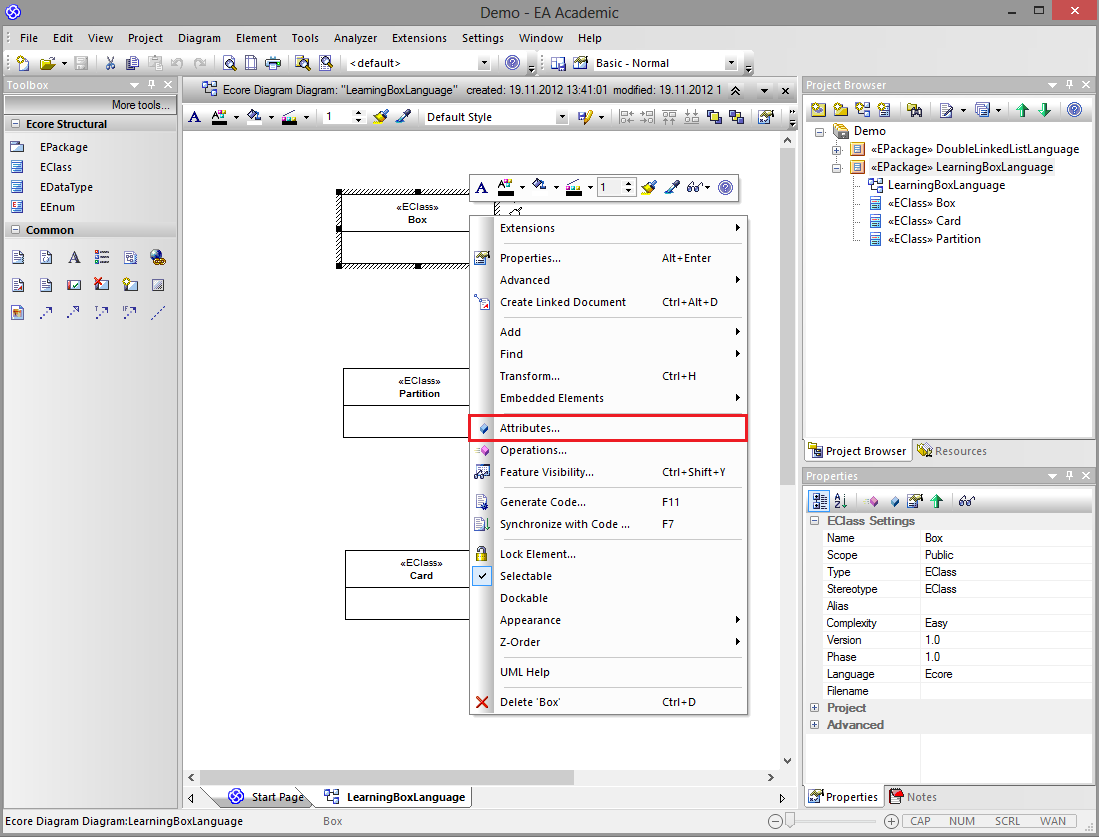
\includegraphics[width=0.7\textwidth]{pics/memBoxBilder/memBox11.png}
	\caption{Context Menu for a class.}
	\label{fig:attribute}
\end{figure}

\clearpage

In the dialogue that pops-up, enter \texttt{name} as the name of the attribute,
choose \texttt{EString} as its type and press \texttt{Save}
(Fig.~\ref{fig:attribute_properties}).  A new attribute for the same class can
be added by choosing \texttt{New}.

\begin{figure}[htbp]
	\centering
  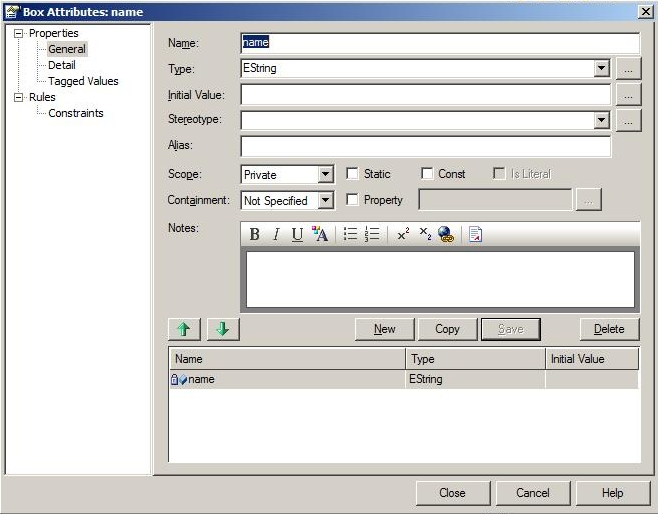
\includegraphics[width=0.7\textwidth]{pics/memBoxBilder/memBox13.png}
	\caption{Adding attributes to a class.}
	\label{fig:attribute_properties}
\end{figure} 

Add attributes to the other classes till your workspace resembles
Fig.~\ref{fig:attribute_completed}.

\begin{figure}[htbp]
	\centering
  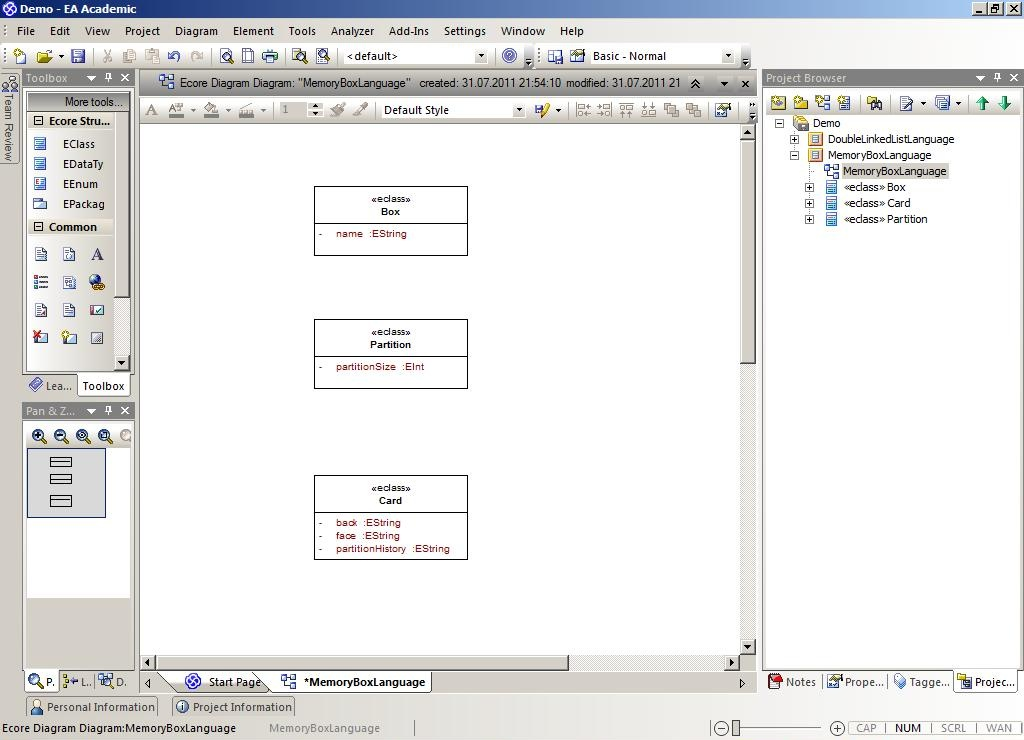
\includegraphics[width=0.73\textwidth]{pics/memBoxBilder/memBox14.png}
	\caption{Main classes with attributes.}
	\label{fig:attribute_completed}
\end{figure}

\clearpage

Now choose \texttt{EPackage} from the toolbox and add it to the current diagram
just like how we added EClasses. Enter \texttt{facade} as the name of the
package. 
 
Ecore supports packages that can be used to structure and group classes
in a metamodel.  In our case, we need  a util class that implements helper
methods for our memory box.  These methods  will be implemented by hand in Java
and the util class thus represents a kind of  interface or ``facade'' between
our model and hand-written code.  We shall soon  see how our Eclipse Plugin
offers extra support if one follows this naming  convention for packages
containing hand-written code. 

To add a class to our new package, first of all create a new diagram in
the package by choosing the \texttt{facade} subpackage and selecting \texttt{New
Diagram} in the Project Browser (Fig.~\ref{fig:epackage_newelement}).

\begin{figure}[htbp]
	\centering
  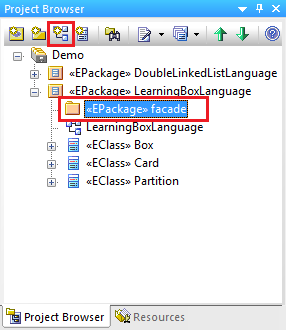
\includegraphics[width=0.5\textwidth]{pics/memBoxBilder/memBox19}
	\caption{Add a class to the package.}
	\label{fig:epackage_newelement}
\end{figure}

In the dialogue that pops-up, choose \texttt{Ecore Diagram} and confirm with
\texttt{OK}.
In the new diagram, create a new class and enter \texttt{MemoryBoxUtil} as its
\texttt{name}.  You can switch between diagrams by choosing the tabs at the
bottom of the screen or by pressing \texttt{alt + } $\Leftarrow$ or
$\Rightarrow$ (Fig.~\ref{fig:epackage_newdiagram}). 

\begin{figure}[htbp] 
	\centering
  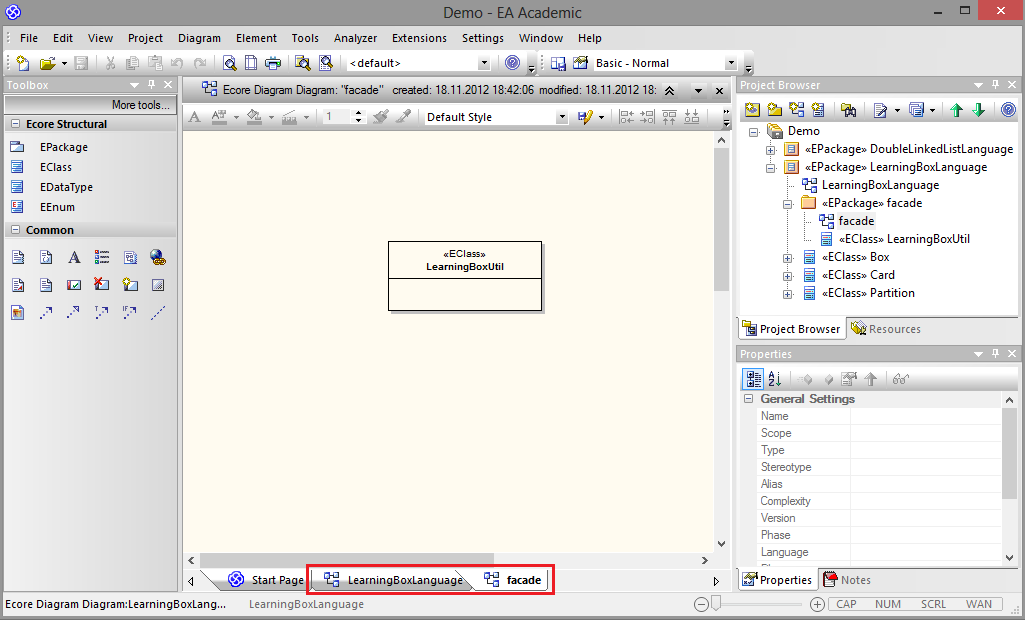
\includegraphics[width=0.55\textwidth]{pics/memBoxBilder/memBox20}
	\caption{Main and subdiagrams in EA.}
	\label{fig:epackage_newdiagram}
\end{figure}
\clearpage 

Your workspace should now resemble Fig.~\ref{fig:epackage_completed}.
Any subpackage like \texttt{facade} can contain diagrams that can be
created and added using the Project Browser. 
In this way an arbitrary nesting of packages and diagrams is possible.

\begin{figure}[htbp]
	\centering
  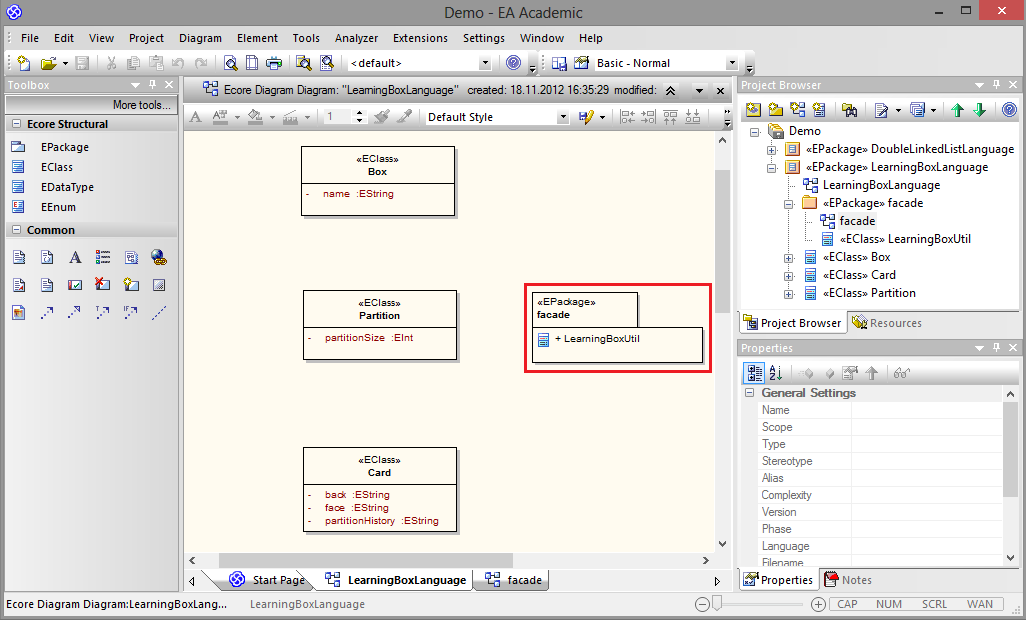
\includegraphics[width=.8\textwidth]{pics/memBoxBilder/memBox22.png}
	\caption{Workspace after adding package and util class.}
	\label{fig:epackage_completed}
\end{figure}

A fundamental gesture in EA is \emph{Quick Link}.  Quick Link is used to create
links between elements in a context sensitive manner.  To use Quick Link,
choose an element and note the little black arrow in its top-right corner
(Fig.~\ref{fig:quicklink}).

\begin{figure}[htbp]
	\centering
  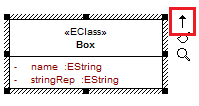
\includegraphics[width=0.4\textwidth]{pics/memBoxBilder/memBox23.png}
	\caption{Quick Link is a central gesture in EA.} 
	\label{fig:quicklink}
\end{figure}

\clearpage 

Now click on the black arrow and pull to another element you wish to ``quick
link" to.  In this case quick link from \texttt{Partition} to \texttt{Box}.  In
the context-menu that pops-up, choose \texttt{EReference}.
(Fig.~\ref{fig:ereference}). 

\begin{figure}[htbp]
	\centering
  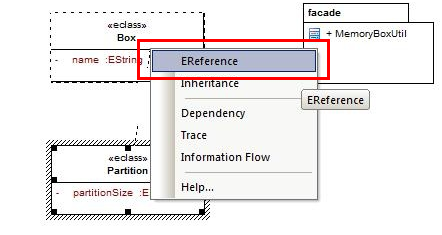
\includegraphics[width=0.6\textwidth]{pics/memBoxBilder/memBox24.png}
	\caption{Create a reference via Quick Link.}
	\label{fig:ereference}
\end{figure}

In the dialogue that pops-up (Fig.~\ref{fig:ereference_properties}), the
direction of the reference can be set.  The default is bidirectional and this is
ok for our \texttt{Box}$\Leftrightarrow$\texttt{Partition} connection.
A \texttt{Name} can also be entered, which is only used for documentation
purposes and is not relevant for codegeneration.

\begin{figure}[htbp]
	\centering
  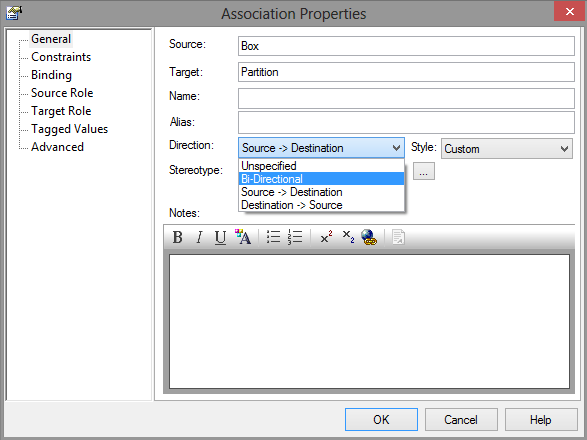
\includegraphics[width=0.6\textwidth]{pics/memBoxBilder/memBox25.png}
	\caption{Enter properties of the reference.}
	\label{fig:ereference_properties}
\end{figure}
	
\clearpage

In the same dialogue choose \texttt{Source Role} and enter the values in
Fig.~\ref{fig:ereference_properties} to set the properties for the ``source''
end of the reference (the \texttt{Box} role).  Important is a name for the role
(\texttt{box}), the \texttt{Multiplicity}, \texttt{Aggregation} and
\texttt{Navigability}.  Repeat the process for the \texttt{Target Role}.
  
\begin{figure}[htbp]
	\centering
  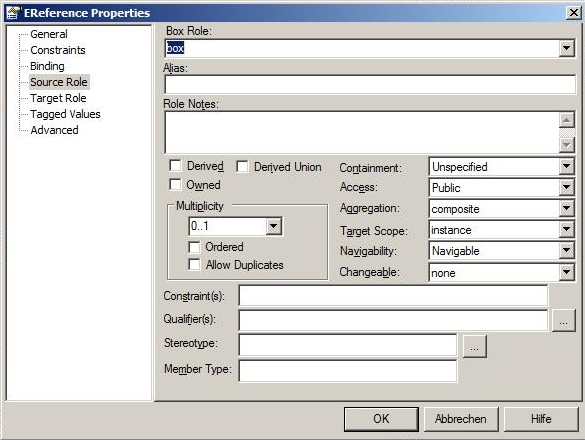
\includegraphics[width=0.5\textwidth]{pics/memBoxBilder/memBox26.png}\\
  \vspace{0.5cm}
  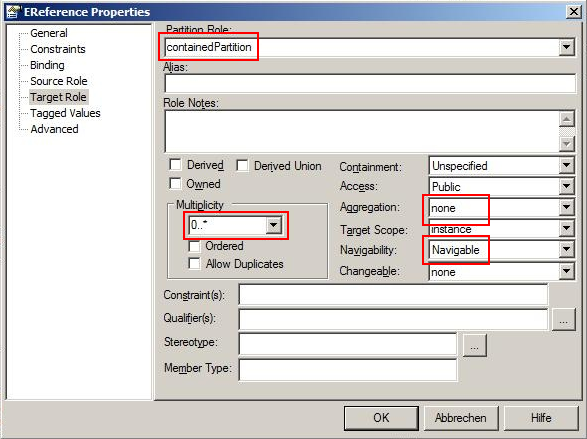
\includegraphics[width=0.5\textwidth]{pics/memBoxBilder/memBox27.png}
	\caption{Enter properties for source and target of reference.}
	\label{fig:reference_ends}
\end{figure}

Navigable ends are mapped to class attributes with getters and setters in Java
and therefore \emph{must} have a specified name and  multiplicity for successful
codegeneration.  
Corresponding values for non-navigable ends can  be regarded as additional
documentation and do not have to be specified.
 
The multiplicity of a reference controls if the relation is mapped to a Java
Collection (\texttt{*},  \texttt{1..*}, \texttt{0..*}), or a single valued class
attribute (\texttt{1}, \texttt{0..1}).

In Ecore, the aggregation values of a reference can either be \texttt{none} or
\texttt{com\-po\-site}.  Composite means that the current role is that of a
\emph{container} for the opposite role.  In our case for example, \texttt{box}
is a container for \texttt{partitions}.\\  This has a series of
consequences: (1) every element must have a container, (2) an element cannot be
in more than one container at the same time, and (3) a container's contents are
deleted together with the container.  Non-composite (\texttt{none}) means that
the current role is not that of a container and the rules for containment do not
hold (reference is a simple ``pointer'').

\clearpage

If you've done everything right, your workspace should now resemble
Fig.~\ref{fig:ereference_completed} with a relation between \texttt{Box} and
\texttt{Partition}.

\begin{figure}[htbp] 
	\centering
  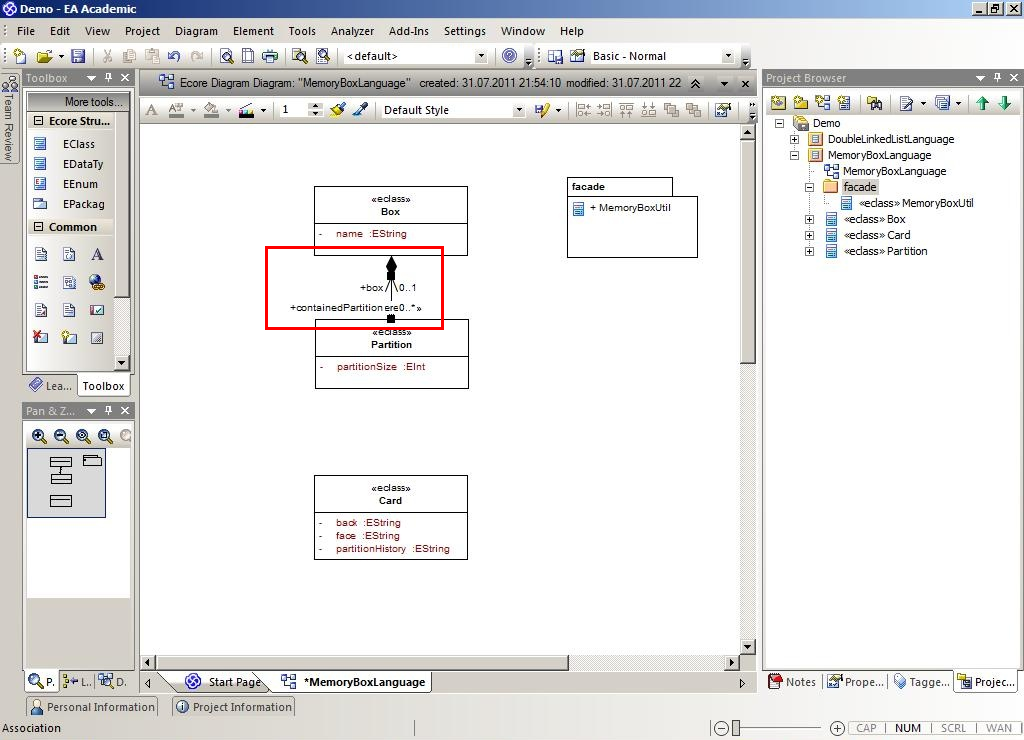
\includegraphics[width=0.7\textwidth]{pics/memBoxBilder/memBox28.png}
	\caption{\texttt{Box} contains \texttt{Partition}s.}
	\label{fig:ereference_completed}
\end{figure}

Create a bidirectional reference\footnote{To be precise, \emph{all} references
in Ecore are actually unidirectional.  A ``bidirectional'' reference in our
metamodel is in reality mapped to two \texttt{EReferences} that are opposites of
each other.  
We however believe it is simpler to handle these pairs as single references and
prefer this concise concrete syntax.} between \texttt{Partition} and \texttt{Card}
and two unidirectional self-references for \texttt{Partition} according to
Fig.~\ref{fig:ereferences_all}\footnote{If you have difficulties deciphering
the role names and other details in the screen shot please refer to
Fig.~\ref{fig:metamodel_complete} for a better diagram of the metamodel.}.
 
\begin{figure}[htbp]
	\centering
  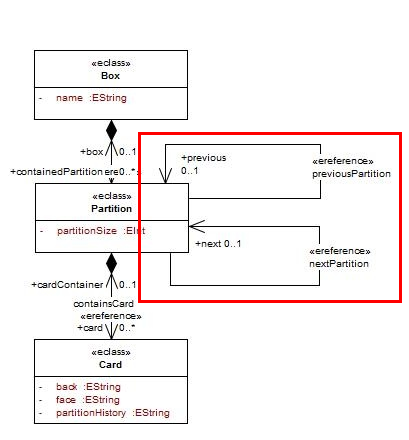
\includegraphics[width=0.5\textwidth]{pics/memBoxBilder/memBox34.png}
	\caption{All relations in our metamodel.}
	\label{fig:ereferences_all}  
\end{figure}

\clearpage

Every system has, in addition to its static structure, certain dynamic aspects
that describe the system's behaviour and how it evolves over time or reacts to
external stimulus.
\marginpar{\emph{Dynamic Semantics}}
In a language, these rules that govern the dynamic behaviour of a system are
referred to collectively as the \emph{Dynamic Semantics} of the language.  
Although these rules can be defined as a set of separate \emph{Model
Transformations}, we take a holistic approach and advocate integrating the
transformations directly in the metamodel as operations.
This fits nicely to the object oriented paradigm and is quite natural in many
cases.  In the next few steps we shall define the \emph{signatures} of some
operations for our memory box.  We will of course use SDMs to \emph{implement}
the methods later.

Right-click \texttt{Partition} to invoke the context-menu depicted in
Fig.~\ref{fig:add_operation} and choose \texttt{Operations\ldots}.

\begin{figure}[htbp]
	\centering
  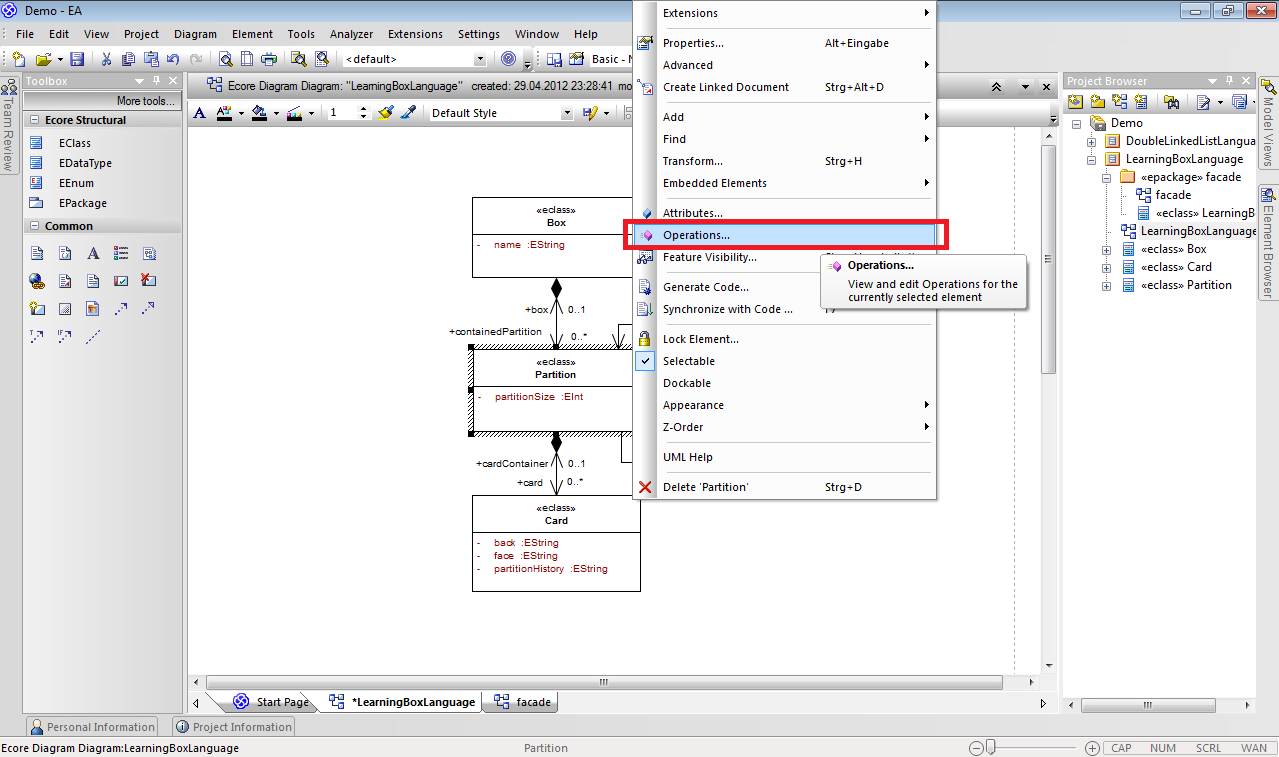
\includegraphics[width=0.6\textwidth]{pics/memBoxBilder/memBox35.png}
	\caption{Add an operation.}
	\label{fig:add_operation}
\end{figure}
 
In the dialogue that pops-up (Fig.~\ref{fig:operation_properties}), enter
\texttt{empty} as the \texttt{Name} of the operation, leave the \texttt{Return
Type} as \texttt{void}.  Press \texttt{Save}.
 
\begin{figure}[htbp]
	\centering
  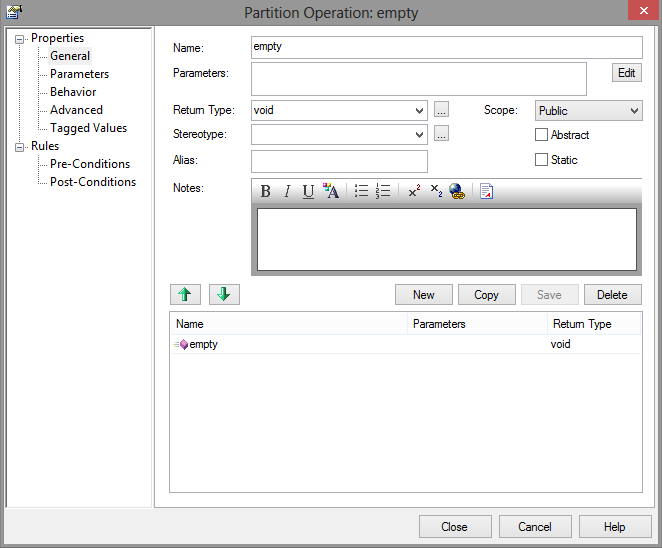
\includegraphics[width=0.45\textwidth]{pics/memBoxBilder/memBox37.png}
	\caption{Properties for operation.}
	\label{fig:operation_properties}
\end{figure}

\clearpage

In the same dialogue, press \texttt{New} to add further operations and enter the
values in Fig.~\ref{fig:operation_parameters}.  Parameters can be added by
pressing \texttt{Edit} and entering the name and choosing the type of each
Parameter in a separate dialogue.

\begin{figure}[htbp]
	\centering
  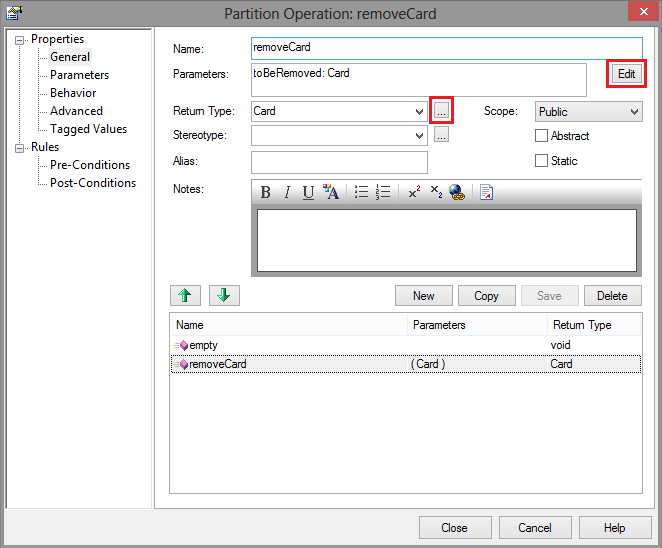
\includegraphics[width=0.53\textwidth]{pics/memBoxBilder/memBox38.png}
	\caption{Parameters and Return Type.}
	\label{fig:operation_parameters} 
\end{figure}

Repeat the process for the values in Fig.~\ref{fig:operation_partition}.  The
\texttt{Return Type} can be chosen via the drop-down menu for primitives
(e.g. \texttt{EBoolean}), or via the \texttt{\ldots} button (indicated in
Fig.~\ref{fig:operation_parameters}) for types in the metamodel
(e.g. \texttt{Card}).

\vspace{-.5cm}
\begin{quote}
$\textbf{Please note:}$ Non-primitive types \emph{must} be chosen via the
\texttt{\ldots} button that allows you to browse for the corresponding elements in your
project.  Just typing them unfortunately won't work due to EA API restrictions!
\end{quote}
\vspace{-.5cm}

If you've done everything right, your dialogue should
now contain three methods \texttt{check}, \texttt{empty}, and
\texttt{removeCard} with corresponding parameters and return types as in
Fig.~\ref{fig:operation_partition}.
\begin{figure}[htbp]
	\centering
  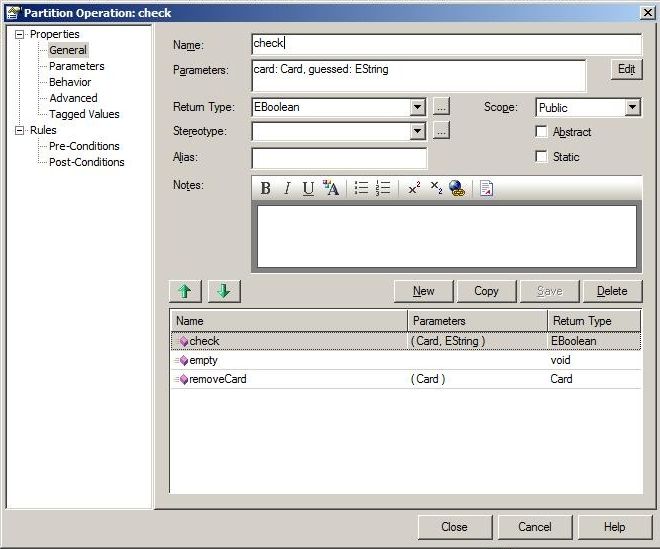
\includegraphics[width=0.53\textwidth]{pics/memBoxBilder/memBox39}
	\caption{All operations in \texttt{Partition}.}
	\label{fig:operation_partition}
\end{figure}
\clearpage

Add all operations analogously for \texttt{Box}, \texttt{Card} and
\texttt{MemoryBoxUtil}, so that your metamodel closely resembles
Fig.~\ref{fig:metamodel_complete}. 
 
\begin{figure}[htbp]
	\centering 
  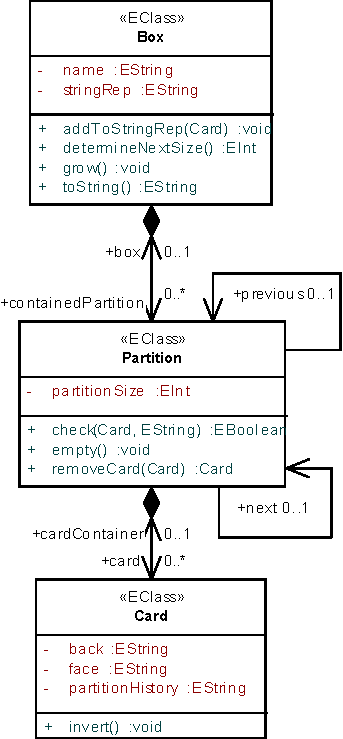
\includegraphics[width=\textwidth]{pics/memBoxBilder/memBox44} 
	\caption{Complete metamodel for our memory box.}
	\label{fig:metamodel_complete}
\end{figure}

Lets take a step back and review our metamodel.  We have modelled a \texttt{Box}
that contains arbitrary many \texttt{Partition}s.  A \texttt{Partition} in the
\texttt{Box} has a \texttt{next} and \texttt{previous} \texttt{Partition} that
can be set or not. Finally, \texttt{Partition}s contain \texttt{Card}s.

A \texttt{Box} has a \texttt{name}, and can be extended by calling
\texttt{grow}. A \texttt{Box} can print out its contents via \texttt{toString}. 
We'll see later in the tutorial why these two methods need our
\texttt{MemoryBoxUtil} as a parameter.

The main method of the memory box is \texttt{Partition::check} that takes a
\texttt{Card} and the user's guess as an \texttt{EString} and returns
\texttt{true} or \texttt{false} depending on if the guess was correct or not.
A \texttt{Partition} can also \texttt{empty} itself of all \texttt{Cards}, or
\texttt{remove} a particular \texttt{Card}.  Last but not least, a
\texttt{Partition} has a \texttt{partitionSize} that can be used to indicate
that the \texttt{Partition} is full and is ready to be revised.

\clearpage

A \texttt{Card} contains the actual content to be learnt as a question on the
card's \texttt{face} and the answer on the card's \texttt{back}. A \texttt{Card}
also maintains a \texttt{partition\-History} which can be used to keep track of
how often a \texttt{Card} has been answered correctly/wrongly.  This might
indicate how difficult the \texttt{Card} is for a specific user.
When learning a language, it makes sense to be able to swap the target and
source langauge and this is supported by \texttt{Card} via \texttt{invert}
(turns the card around).

Now try to export the metamodel for codegeneration in Eclipse.  To do this
right-click on \texttt{MemoryBoxLanguage} and choose ``Add-In/MOFLON::Ecore
Addin/Export Selection to Workspace''.  Then switch to your Eclipse work\-space
and refresh the metamodel workingset.

If you have done everything right, a new project \texttt{MemoryBoxLanguage}
should be created in the \texttt{Demo} working set in your Eclipse workspace.
If this is not the case please ensure that your metamodel is identical with
Fig.~\ref{fig:metamodel_complete}.  If you believe everything is correct and
things still don't work then feel free to contact us at
\href{mailto:contact@moflon.org}{contact@moflon.org}.  If code is generated
successfully, take a look at all the stuff that has been generated under
\texttt{/gen}, especially the default  implementation for all methods that just
throws an  \texttt{OperationNotSupported} exception.  We shall see later in the
tutorial  that the EMF codegenerator actually supports merging hand-written
implementations of methods with generated code.  With eMoflon however, we can
also model a large part of the dynamic semantics and only need to implement
small helper methods for e.g. string manipulation by hand.

Let's move on and model the dynamic behaviour of our memory box!